\chapter{Statistical Treatment and Markov Chain Monte Carlo}
\label{chap:mcmc}

\epigraph{There are three kinds of lies: lies, damned lies, and statistics}{Mark Twain}

The analysis presented in this thesis employs a Bayesian view of statistics, in which the end result is a posterior probability distribution $P(\vec{\theta}|D)$ for the model $\vec{\theta}$ given the observed data $D$. It is built from the joint probability distribution of observing data $D$ given the model $\vec{\theta}$, $P(D|\vec{\theta})$, provided some prior information on $\vec{\theta}$, $P(\vec{\theta})$. These quantities are related through Bayes' theorem,

\begin{equation}
P(\vec{\theta}|D) = \frac{P(D|\vec{\theta})P(\vec{\theta})}{\int P(D|\vec{\theta})P(\vec{\theta})d\vec{\theta}}
\label{eq:bayes}
\end{equation}
which is conditional on the full model space. The $P(D|\vec{\theta})$ from the event distributions are modelled with a Poisson probability distribution for the data $n$ being a fluctuation of the simulation $\lambda(\vec{\theta})$ which is dependent on the model $\vec{\theta}$. The $P(\vec{\theta})$ is the prior knowledge of the model $\vec{\theta}$ from data not used in this analysis (e.g. external hadron scattering data, cosmic data at ND280) and is modelled using a multivariate Gaussian probability distribution. Each parameter $i$ has a central value $\mu_i$ which is varied to $X_i$ during the MCMC sampling and is related to parameter $j$ through the covariance matrix $\mathbf{V}_{ij}$. This is formally expressed as

\begin{equation}
	P(D|\vec{\theta}) P(\vec{\theta}) = \prod \mathcal{L}_\text{Total} = \prod \left(\mathcal{L}_\text{Samples} \times \mathcal{L}_\text{Systematics}\right)
\end{equation}

or more conveniently in the logarithmic space,
\begin{equation}
\label{eq:test_stat}
\begin{split}
	- \log\mathcal{L}_\text{Total} = &\sum_\text{Bins} \left[ \lambda(\vec{\theta}) - n + n \log \frac{n}{\lambda(\vec{\theta})} \right] + \\
									& \sum_\text{Systematics} \frac{1}{2} \left[ ( X_i - \mu_i ) \left( \boldsymbol{V} \right)^{-1}_{ij} ( X_j - \mu_j ) \right]
\end{split}
\end{equation}

In practice, the posterior is generally not analytically solvable and $\vec{\theta}$ might be of very high dimension---in this thesis we have $\text{dim}(\vec{\theta})=687, 1209, 4369$. It is instead commonplace to sample from the posterior using Monte Carlo methods\cite{bayesian_tutorial}, producing a density of points proportional to the posterior, correct up to a normalising factor.

Markov Chain Monte Carlo methods have been used extensively in astro-statistics, computational physics and biology, and is central to evaluating the multi-dimensional integrals that occur in Bayesian statistics. The necessary and sufficient conditions for a Markov Chain  successfully constructing the posterior density requires
\begin{itemize}
	\item \textbf{Irreducibility:} From any given state, the probability to reach any other state has to always be non-zero
	\item \textbf{Recurrence:} When the stationary distribution has been found, all subsequent steps must sample from that stationary distribution
	\item \textbf{Aperiodicity:} The sequence of steps must not be periodic
\end{itemize}
A detailed discussion of these criteria can be found in \cite{mcmc_practice, mcmc_handbook}.

\section{The Metropolis-Hastings Algorithm}
This analysis uses the well established Metropolis-Hastings algorithm\cite{metropolis,hastings} to explore the parameter space $\vec{\theta}$ and sample the posterior $P(\vec{\theta}|D)$. It can be considered a random walk which steers towards areas of high probability in \autoref{eq:test_stat}. The algorithm consists of a set of steps which are repeated $N$ times:
\begin{itemize}
	\item \textbf{Initialisation}: A random starting point of the parameters $\vec{\theta}$ is chosen
	\item \textbf{Step proposal}: A new set of parameters $\vec{\theta}'$ is proposed using a proposal function, symmetric around the previous accepted point
	\begin{equation}
		\vec{\theta}' = \vec{\theta}+\text{rand}_{\text{Proposal Funct.}}(\vec{\theta})
	\end{equation}
	The proposal function may have tuneable size, which can increase or decrease the acceptance rate but can significantly worsen the parameter space exploration.
	\item \textbf{Acceptance probability}: The total test-statistic (\autoref{eq:test_stat}) is calculated for the current and proposed step, whose likliehood ratio forms the acceptance probability
	\begin{equation}
		\alpha = \min \left[ 1, \exp\left(\log\mathcal{L}_\text{Total}(\vec{\theta}) - \log\mathcal{L}_\text{Total}(\vec{\theta}') \right)\right]
	\end{equation}
	\item \textbf{Accept or reject}: A uniform random number $u \in U[0,1]$ is selected and compared to $\alpha$, which determines if the new parameter set $\vec{\theta}'$ is accepted or rejected
	\begin{equation}
	\vec{\theta} =
	\begin{cases}
		\vec{\theta}' & \alpha \ge u \\
		\vec{\theta} & \alpha < u
	\end{cases}
	\end{equation}
	\item \textbf{Repeat}: Repeat step proposal
\end{itemize}
Importantly, the Metropolis-Hastings algorithm will always accept steps in the direction of higher probability, but also accepts steps with lower probabilities. Thus an adequately explored MCMC does not suffer from local minima and scales relatively well with increasing dimensionality. However, after $N$ steps there is no guarantee that the posterior has been adequately sampled and the parameters have converged. There general guidance on how big $N$ should be is as large as possible\cite{mcmc_handbook}.

\begin{figure}[h]
	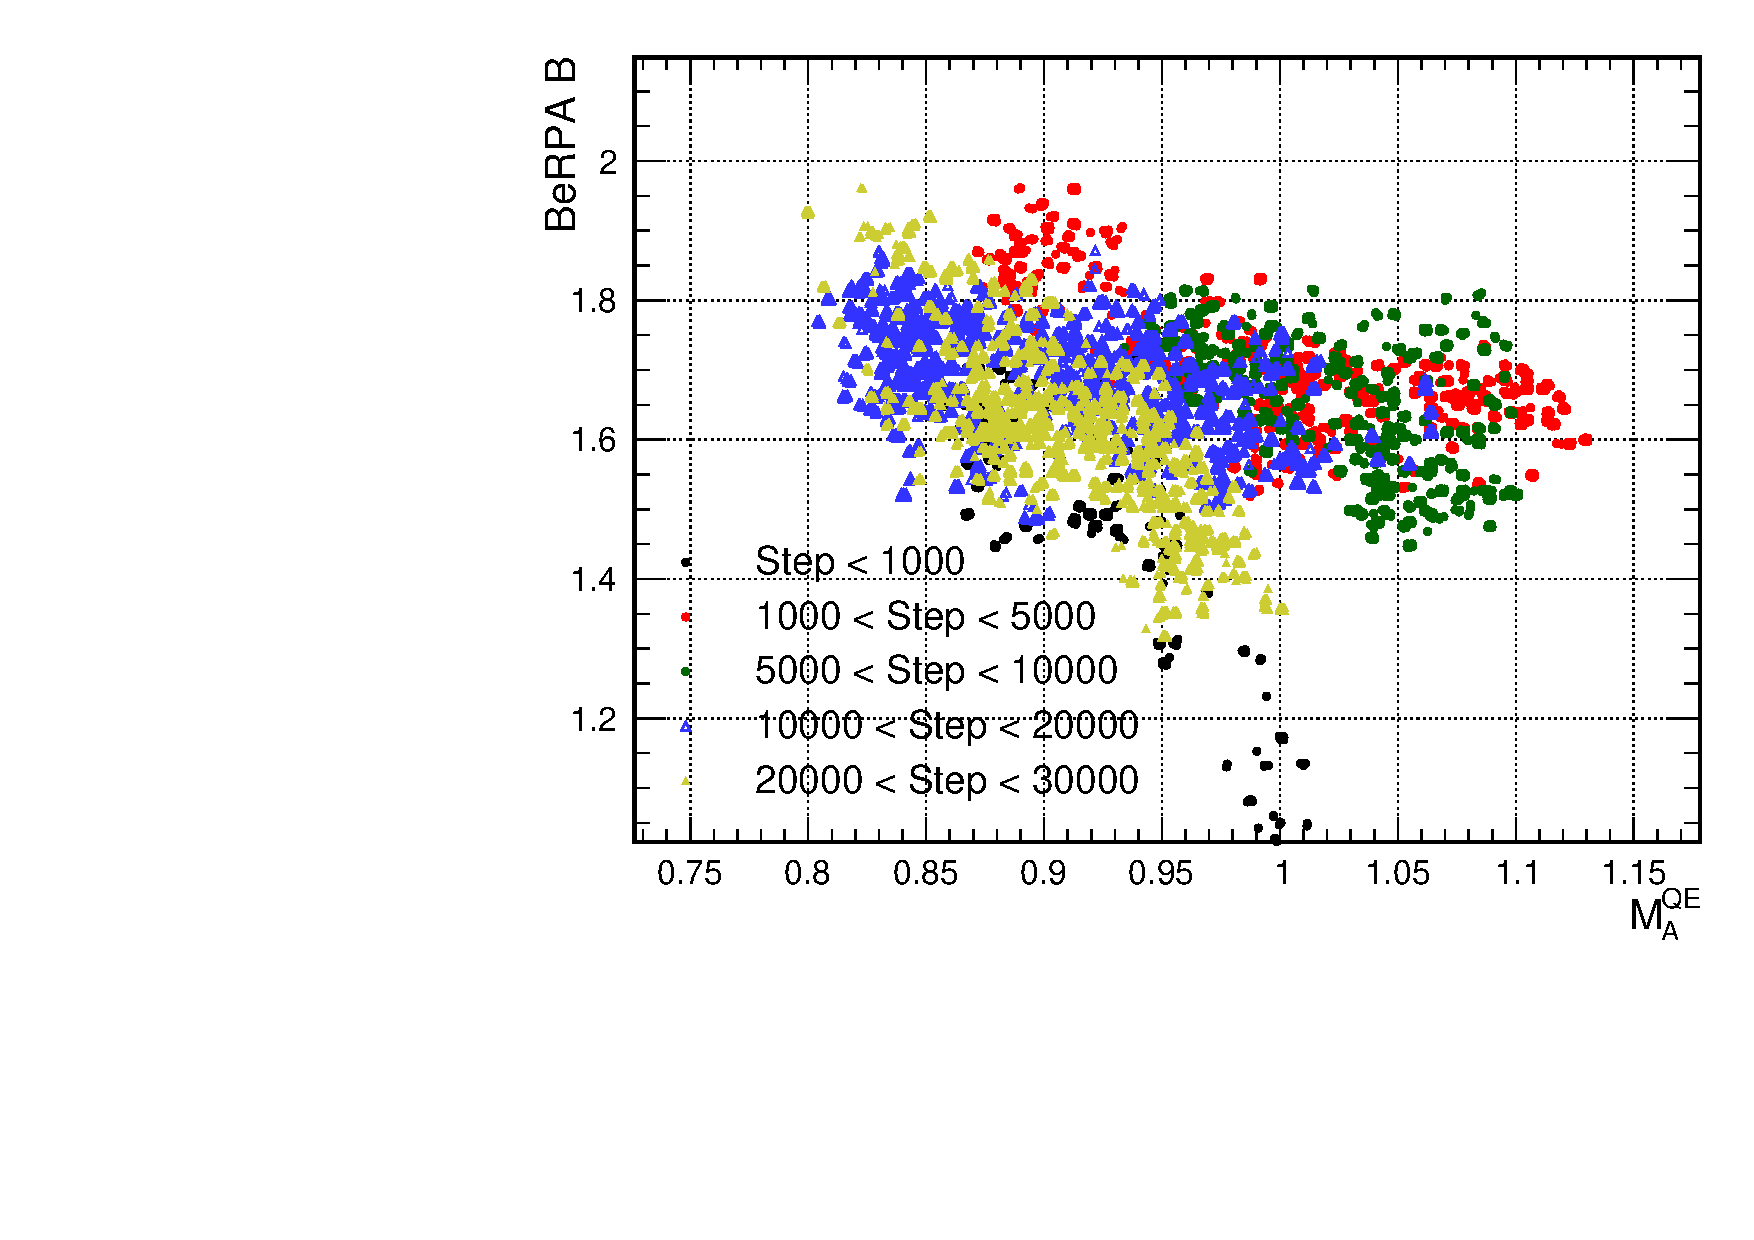
\includegraphics[width=0.6\textwidth, trim={0mm 0mm 0mm 0mm}, clip,page=1]{figures/mcmc/corr_maqe_berpab}
	\caption{Evolution of two correlated interaction parameters with MCMC step for a fit to data at ND280}
	\label{fig:corr_evo}
\end{figure}
\autoref{fig:corr_evo} shows the evolution of two correlated interaction parameters, detailed in \autoref{subsec:syst_xsec}. The MCMC initially starts at $\{M_A^{QE}, \text{BeRPA B}\} \sim \{1.0, 1.1\}$ but the region is disfavoured by the test-statistic. After only 1,000 steps the BeRPA B parameter has roughly reached stationarity, whereas $M_A^{QE}$ is exploring up to $\sim20,000$ steps.

Since separate MCMC are statistically independent once they've reached stationarity, they can be combined to lower MC statistical error in the sampling with better point and interval estimates. Hence MCMC is commonly run in parallel: for ND280-only fits we often use at least three, whereas full ND280+SK oscillation fits run several hundred.

\section{Diagnostics}
The main tuneable parameters in a Metropolis-Hastings algorithm are the step-sizes of the proposal functions and the number of steps $N$. The MCMC variables are tuned until convergence in the parameters are obtained. For this analysis a set of diagnostics are used for monitoring convergence: parameter traces, likelihood traces, batched means and autocorrelations, as recommended in literature\cite{mcmc_handbook}.

The traces are simply the parameter values with each MCMC step, which is a function of the step-size of the Gaussian proposal function. Too fine step-sizes cause high acceptance probability with poor parameter space exploration and highly correlated steps, with the opposite true for coarse step-sizes. The optimal acceptance probability is 0.234\cite{step_prop,mcmc_handbook} and step-size tuning is done as to roughly coincide with this number.

The batched means are similar to the traces but cuts up the steps into batches and compares the average parameter values in each batch. This is typically a good indicator of burn-in, as small batches near the start of the chain may have different values to batches near the end of the chain.

The auto-correlation function $r_k$ after lag $k$ steps is identical to that in signal processing,
\begin{equation}
r_k = \frac{\sum_{i=1}^{N-k}\left(Y_i-\bar{Y}\right) \left(Y_{i+k} - \bar{Y}\right)} {\sum_{i=1}^N \left(Y_i-\bar{Y}\right)^2 }
\end{equation}
and is a measure of how correlated a step is with the $k$ steps ahead. This is an important tool for MCMC to diagnose chain stability, since the optimal acceptance probability of 0.234 can be easily achieved by varying the step-sizes, although this can incur significant step-to-step correlations, which the auto-correlation measure calculates. Generally, this analysis aims to have auto-correlations of less than 0.2 after lag $k=10,000$. \autoref{fig:auto_corr} shows example auto-correlation functions for a chain which did not pass this criteria in the interaction parameters, so was step-size tuned further.
\begin{figure}[h]
	\begin{subfigure}[t]{0.44\textwidth}
		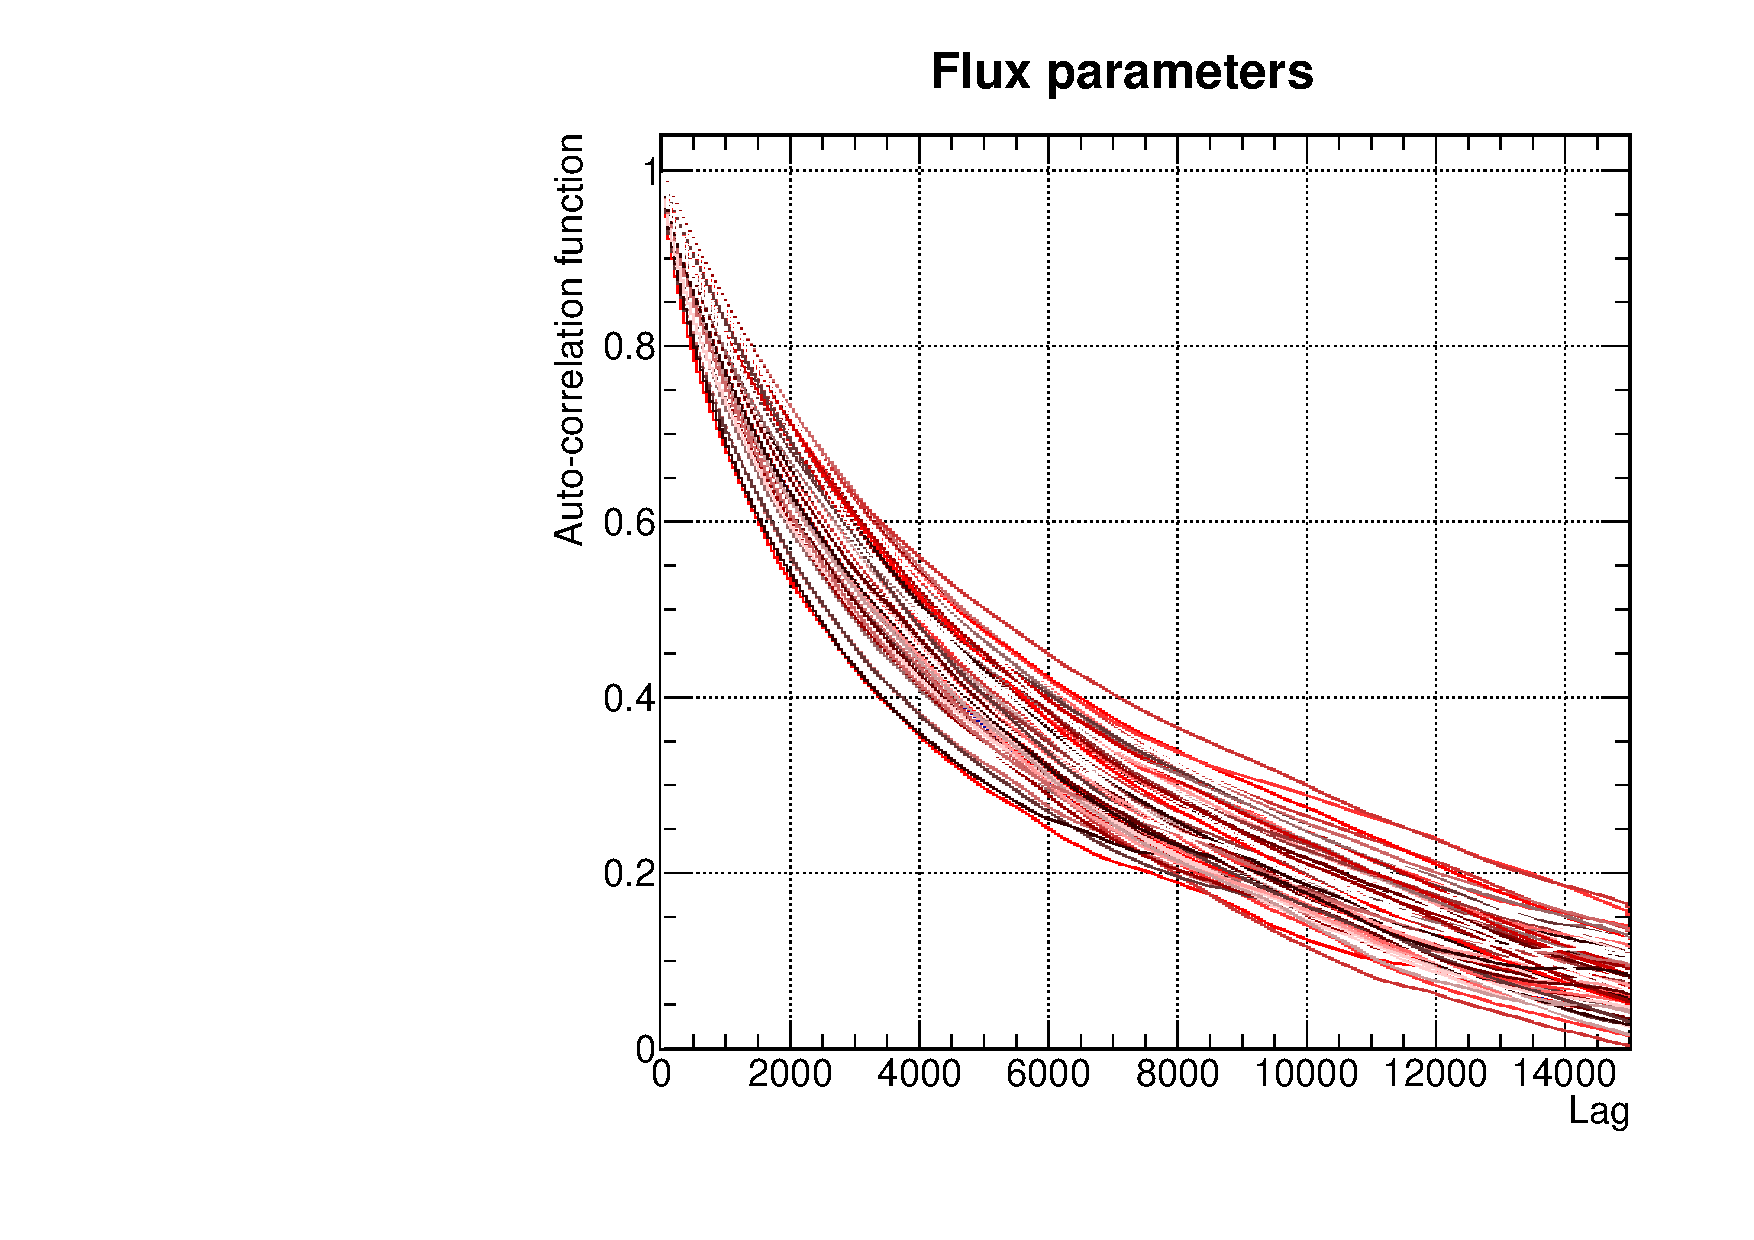
\includegraphics[width=\textwidth, trim={0mm 0mm 0mm 0mm}, clip,page=1]{figures/mcmc/2018a_MultiPi_Binningv6_NewCov_Data_merge_MCMC_diag}
	\end{subfigure}
	\begin{subfigure}[t]{0.44\textwidth}
		\includegraphics[width=\textwidth, trim={0mm 0mm 0mm 0mm}, clip,page=2]{figures/mcmc/2018a_MultiPi_Binningv6_NewCov_Data_merge_MCMC_diag}
	\end{subfigure}
	\caption{Auto-correlation functions for an example fit to ND280 data}
	\label{fig:auto_corr}
\end{figure}

In the case where multiple MCMC have sampled the same posterior we also compare the above diagnostics chain to chain. In the case of suspected non-convergence after significant number of steps the $\hat{R}$ test\cite{gelman_rubin} is also used, which estimates the improvement in parameter variance that may be achieved by running a chain for longer.

\section{Burn-in}
Since the initial parameters $\vec{\theta}$ aren't necessarily in a region of high probability density, it generally takes an MCMC some time to reach the stationary posterior distribution. This parameter exploration period is normally referred to as the ``burn-in'' period of a MCMC and is usually discarded. \autoref{fig:2p2h_shape_mcmc} shows the evolution of a parameter present in the analysis with step for six separate MCMCs, all starting with the parameter value around 0. 
\begin{figure}[h]
	\begin{subfigure}[t]{0.40\textwidth}
		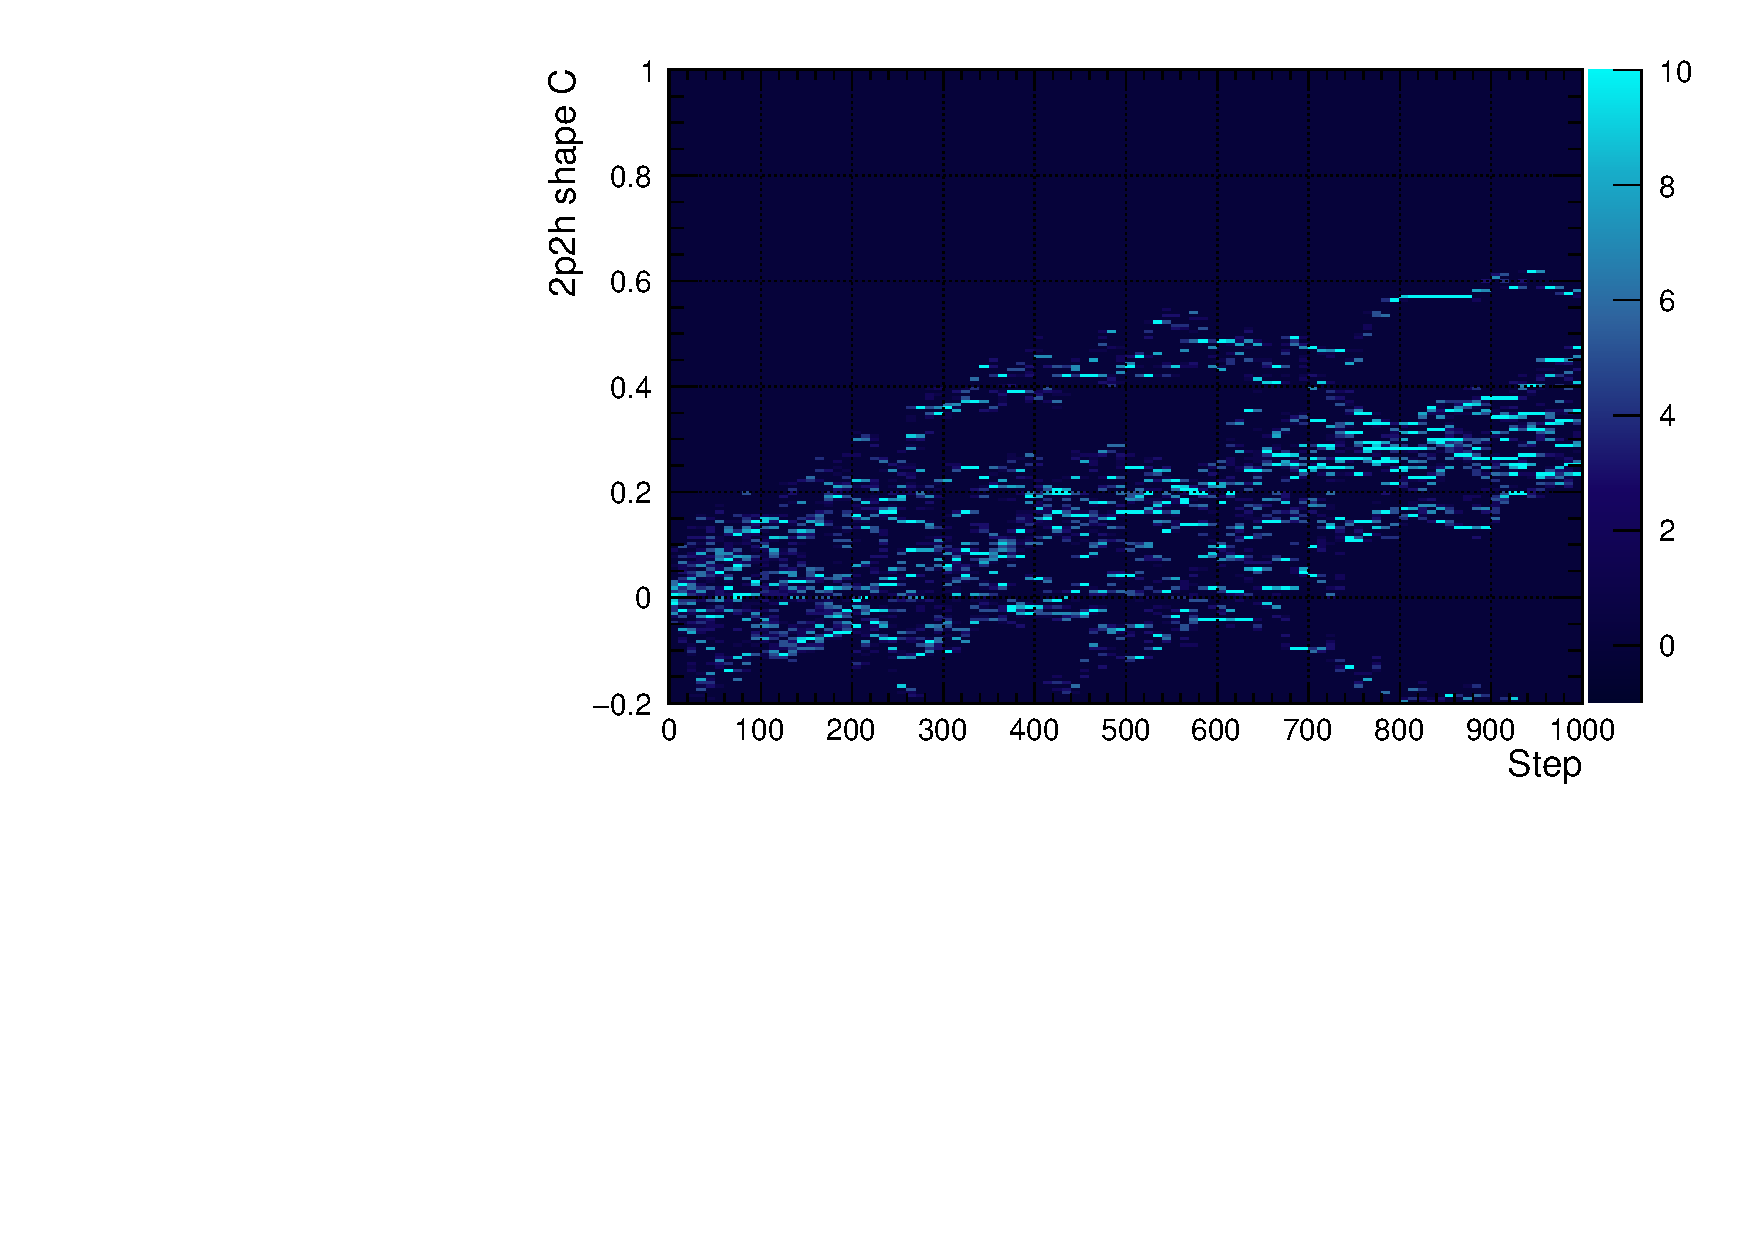
\includegraphics[width=\textwidth, trim={0mm 0mm 0mm 0mm}, clip,page=1]{figures/mcmc/2p2h_shape_C_step}
	\end{subfigure}
	\begin{subfigure}[t]{0.40\textwidth}
		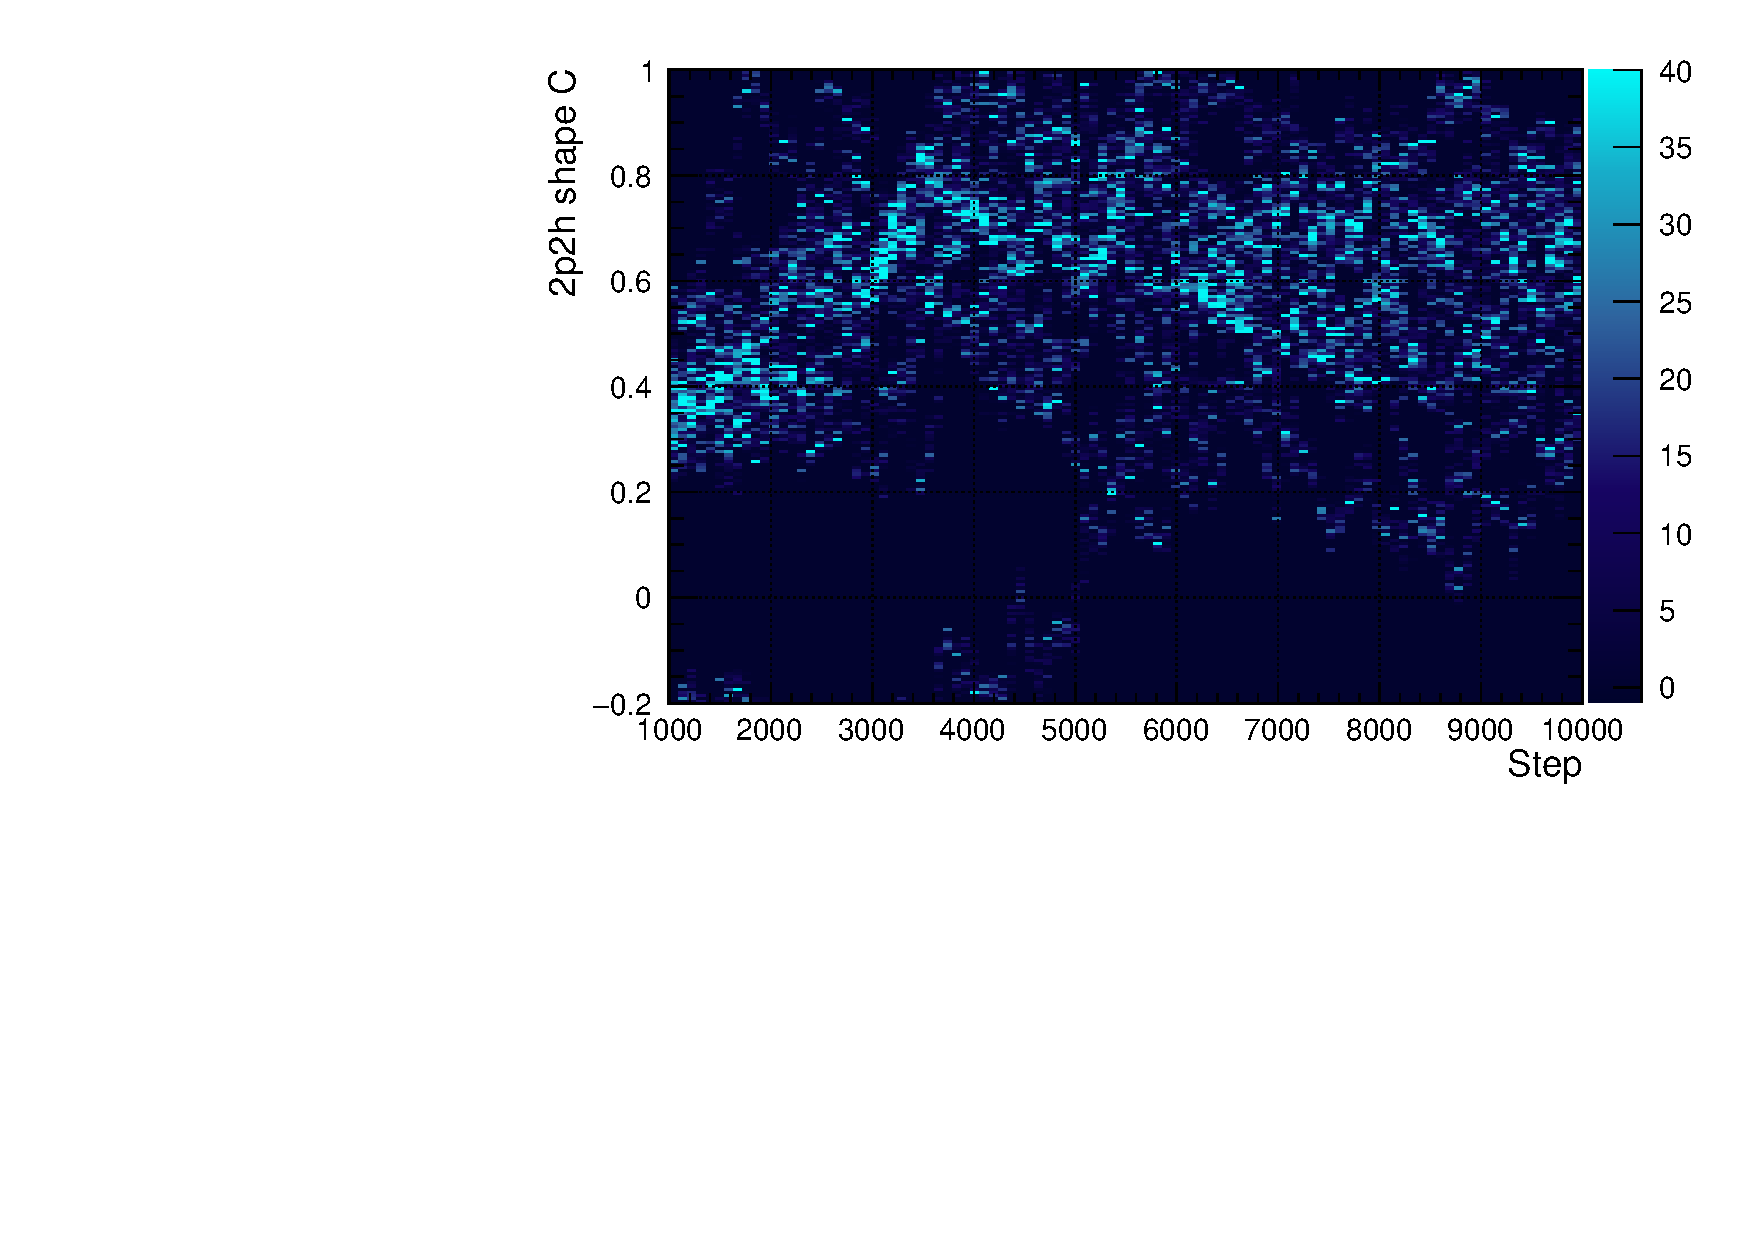
\includegraphics[width=\textwidth, trim={0mm 0mm 0mm 0mm}, clip,page=1]{figures/mcmc/2p2h_shape_C_step2}
	\end{subfigure}
	
	\begin{subfigure}[t]{0.40\textwidth}
		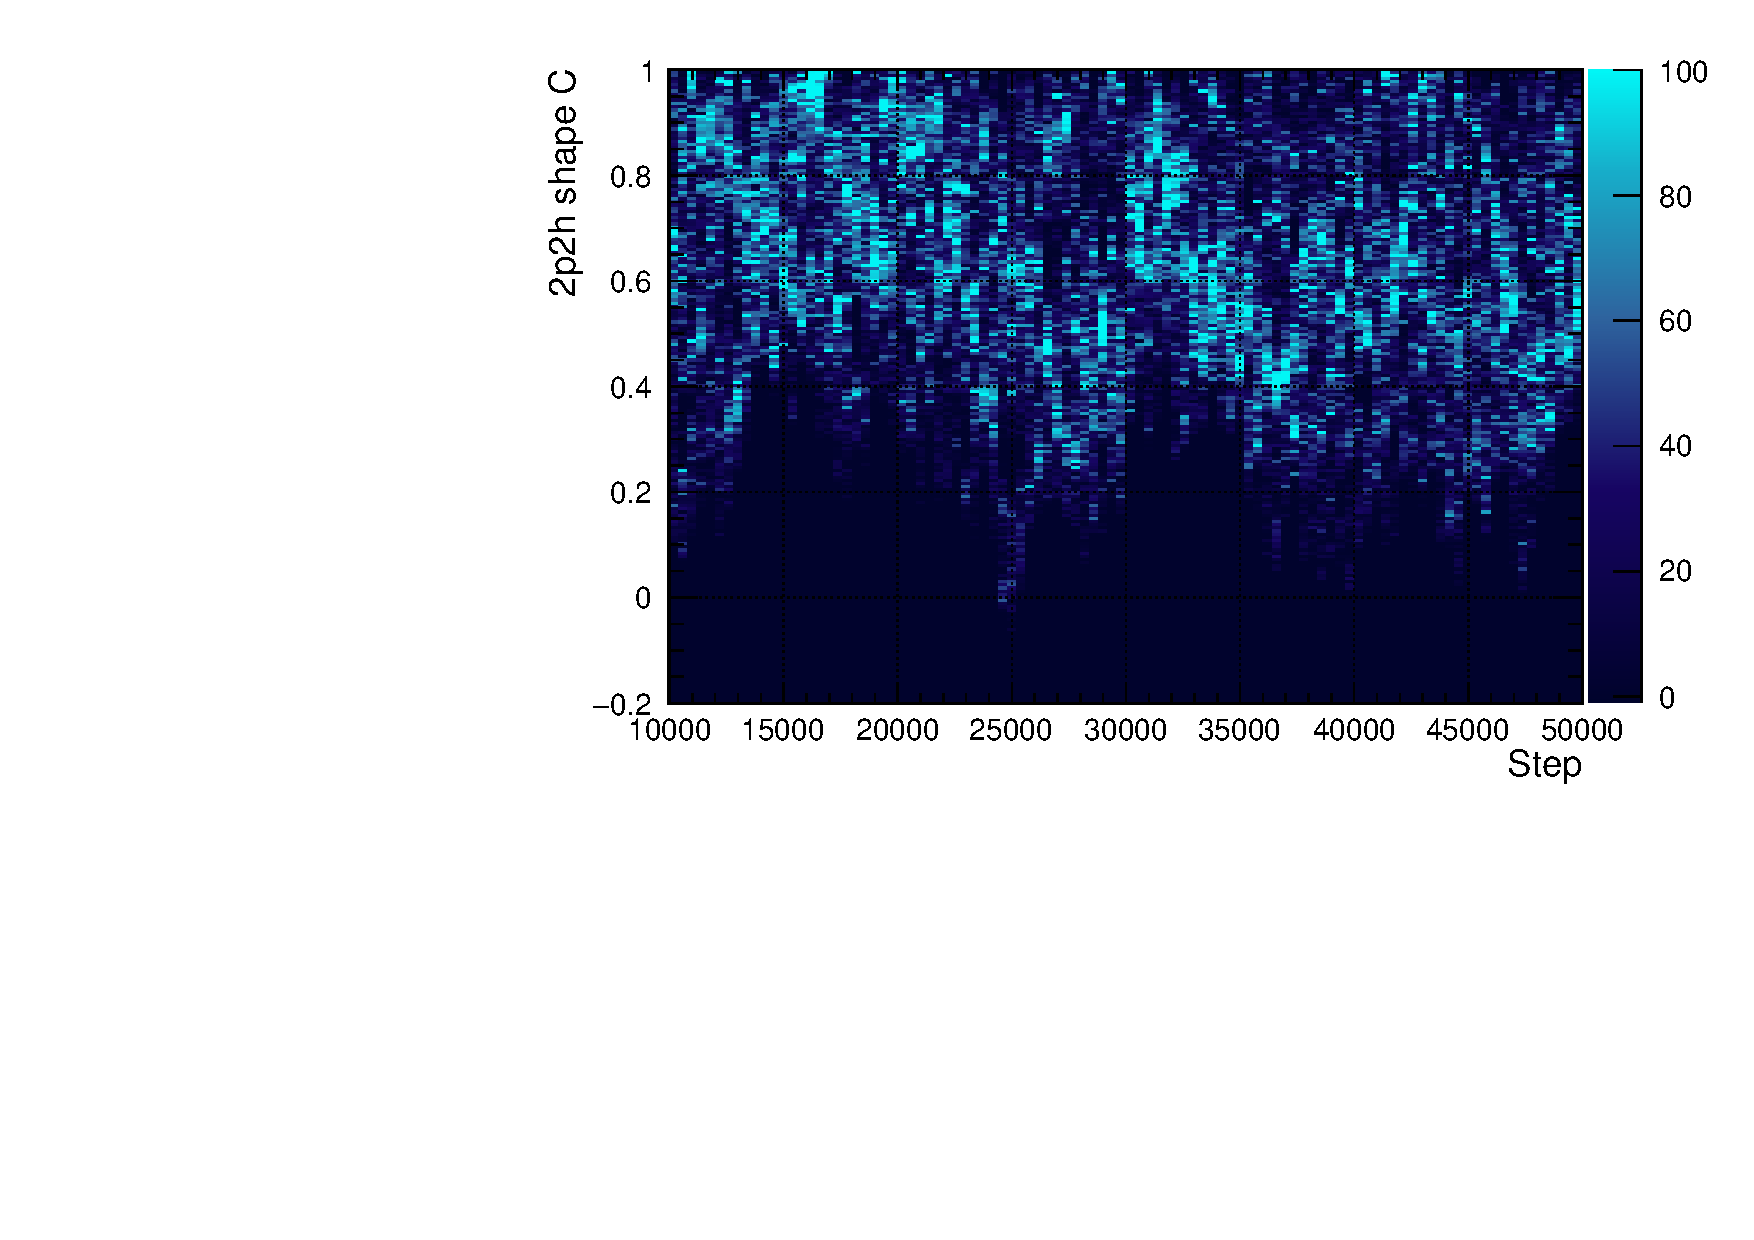
\includegraphics[width=\textwidth, trim={0mm 0mm 0mm 0mm}, clip,page=1]{figures/mcmc/2p2h_shape_C_step3}
	\end{subfigure}
	\begin{subfigure}[t]{0.40\textwidth}
		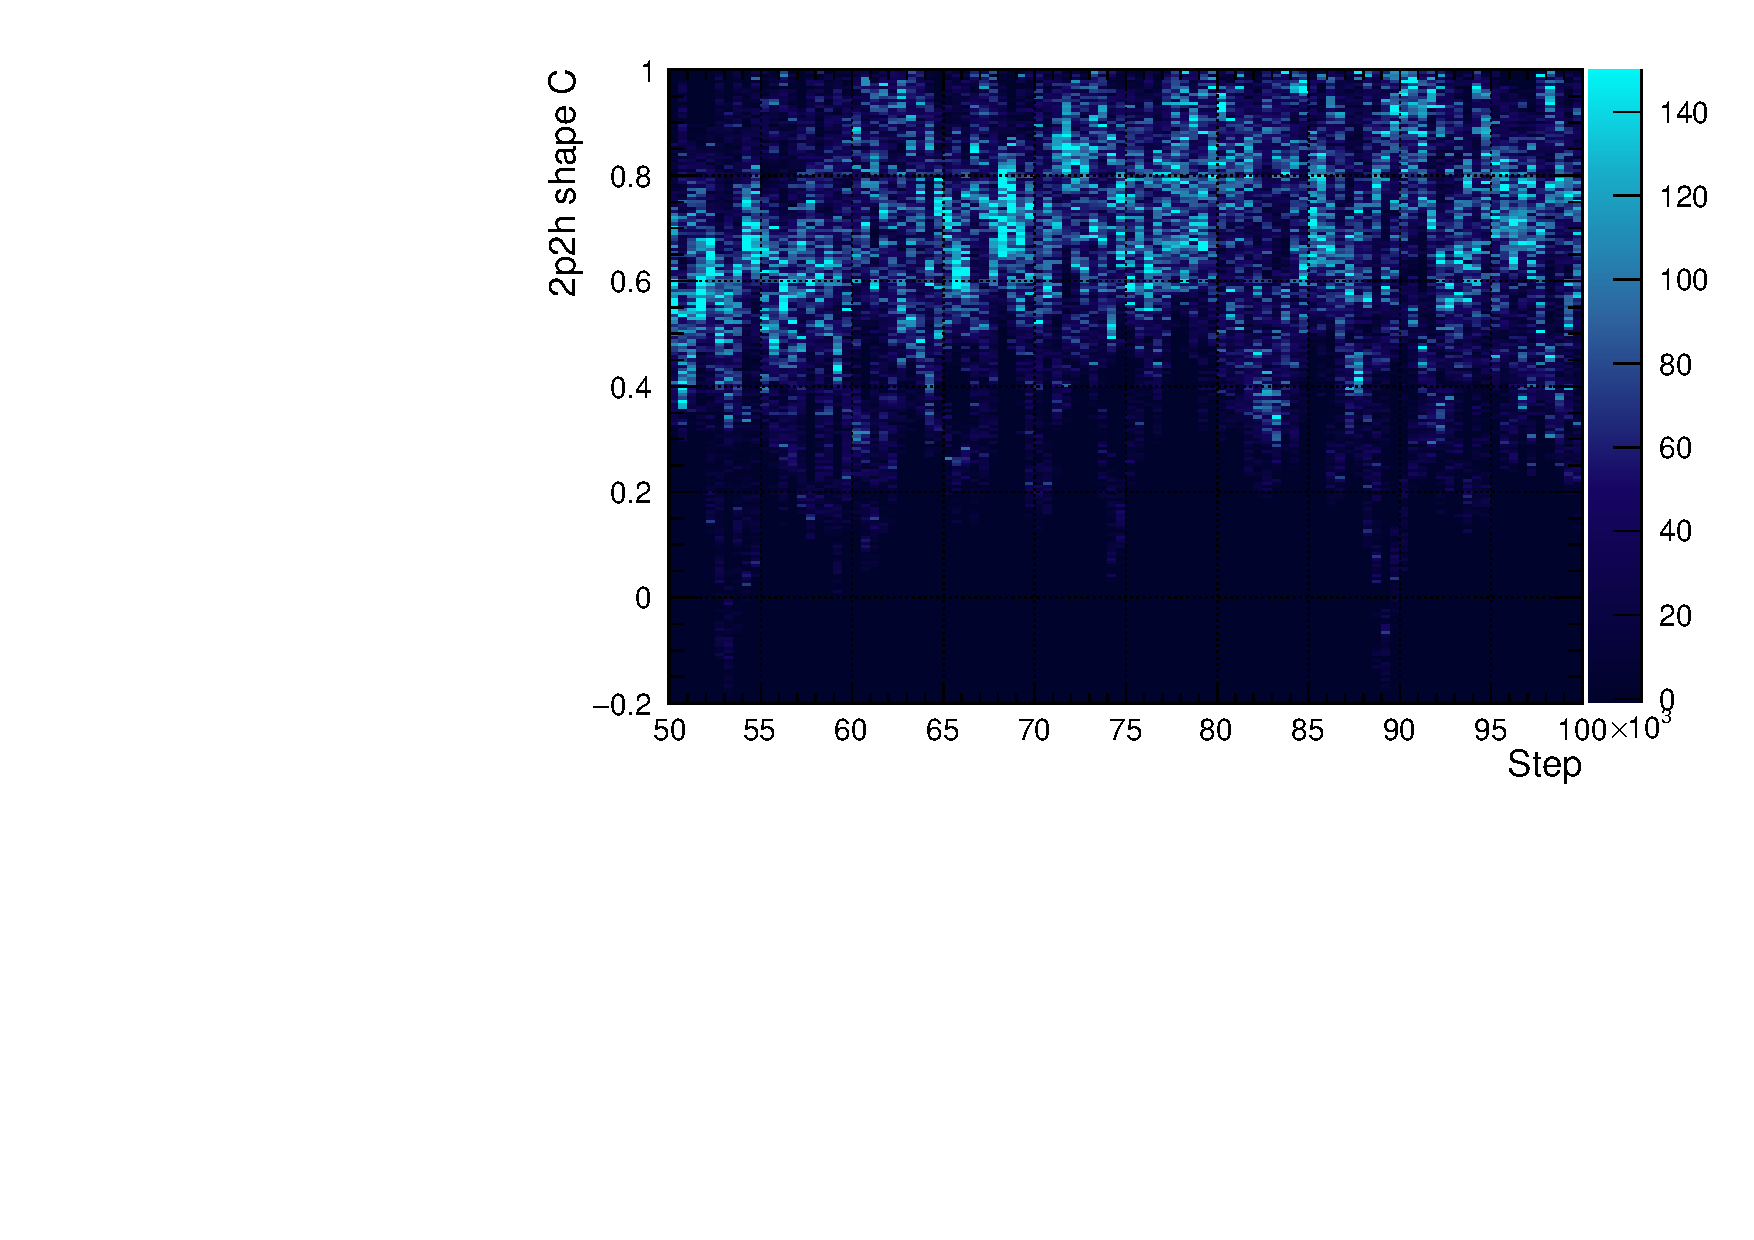
\includegraphics[width=\textwidth, trim={0mm 0mm 0mm 0mm}, clip,page=1]{figures/mcmc/2p2h_shape_C_step4}
	\end{subfigure}
	\caption{2p2h shape C evolution over the number of steps with six separate chains}
	\label{fig:2p2h_shape_mcmc}
\end{figure}

The chains appear to converge after 30,000 steps, which would indicate an approximate burn-in. The auto-correlations are also checked, along with a random subset of other parameters. The total test-statistic in \autoref{eq:test_stat} is also checked over steps, and in this case results in \autoref{fig:llh_step}. All chains initially walk towards the minimum and reach it after about 800 steps. The chains then globally step out of the minimum and explore the area around it, which appears stable after 20,000 steps.
\begin{figure}[h]
	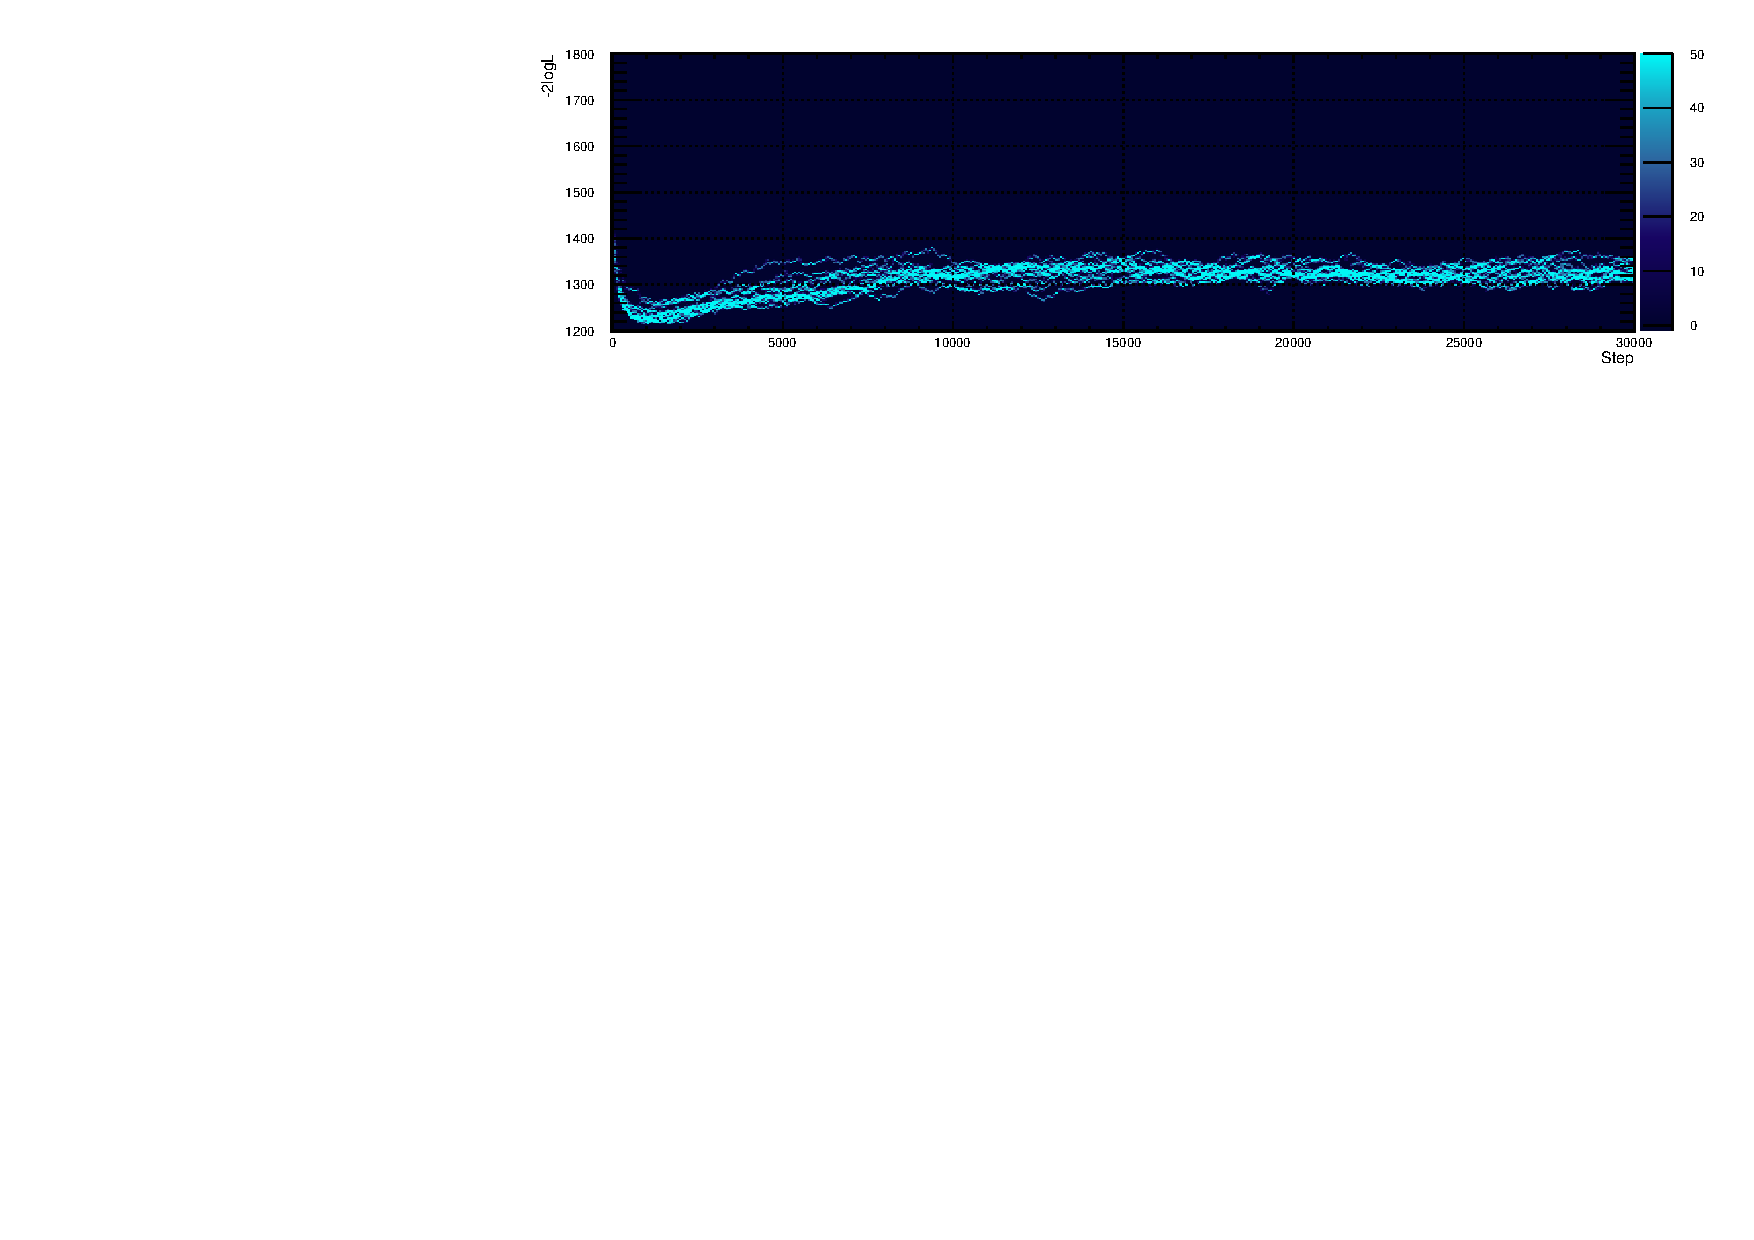
\includegraphics[width=\textwidth, trim={0mm 0mm 0mm 0mm}, clip,page=1]{figures/mcmc/logl_step0}
	\caption{Test-statistic evolution over the steps for six separate chains}
	\label{fig:llh_step}
\end{figure}

The analyses presented in this thesis use a more conservative approach than above since computational power was not an issue. Generally, individual chains are at least 1,000,000 steps long and at least three such chains are run in parallel and the burn-in is always at least 1/4th of the total.

\section{Point Estimates and Uncertainties of Parameters}
This analysis propagates a full high-dimensional posterior---rather than central values with uncertainties related through a covariance matrix---so is less concerned with the accuracy of point estimates and their uncertainties. Furthermore, the posterior only contains parameters considered as nuisance parameters in oscillation analyses. This saves significant computational time, since point estimation in high dimensions with correlated parameters requires a significant number of MCMC steps or a better suited algorithm than Metropolis-Hastings.

However, many point estimates with uncertainties are presented in this work, especially when validating against the frequentist ``BANFF'' framework in \autoref{chap:banff_valid}.
 
\subsection{Parameters of Interest and Marginalisation}
At minimum, 73 parameters are propagated to oscillation analyses in this work. Hence the number of parameters of interest is high, and visualising parameter behaviour becomes difficult. Throughout the ND280 fits we project the high-dimensional posterior onto one or two dimensions---the latter being used to form the covariance matrices. The projection uses the marginalisation method, in which we integrate out the posterior's dependency on all but the single ``parameter of interest''. Naturally, this process loses information about the full posterior, so is not propagated to the SK analysers.

Consider the single parameter of interest $x$ where $x \in \vec{\theta}$ and the remaining parameter space is denoted $\vec{\theta}'$. The marginalised posterior density of the parameter $x$ given the data $D$, $P(x|D)$, is simply given by
\begin{equation}
P(x|D) = \int P(\vec{\theta}',\vec{x}|D) d\vec{\theta}'
\end{equation}

This one-dimensional posterior distribution is used to obtain point estimates and uncertainties. We use chiefly three methods:
\begin{itemize}
	\item The arithmetic mean and rms
	\item The fitted Gaussian mean and 1$\sigma$
	\item The highest posterior density with (a)symmetric errors
\end{itemize}
The three methods are used to flag when posteriors have non-Gaussian shapes, since in the Gaussian case the above are all equivalent. This can for example happen for parameters that have hard cut-offs, strong correlations, and for parameters that are switches (``on'' or ``off''). \autoref{fig:point_estimate} demonstrates the differences between the methods for a non-Gaussian beam parameter.
\begin{figure}[h]
	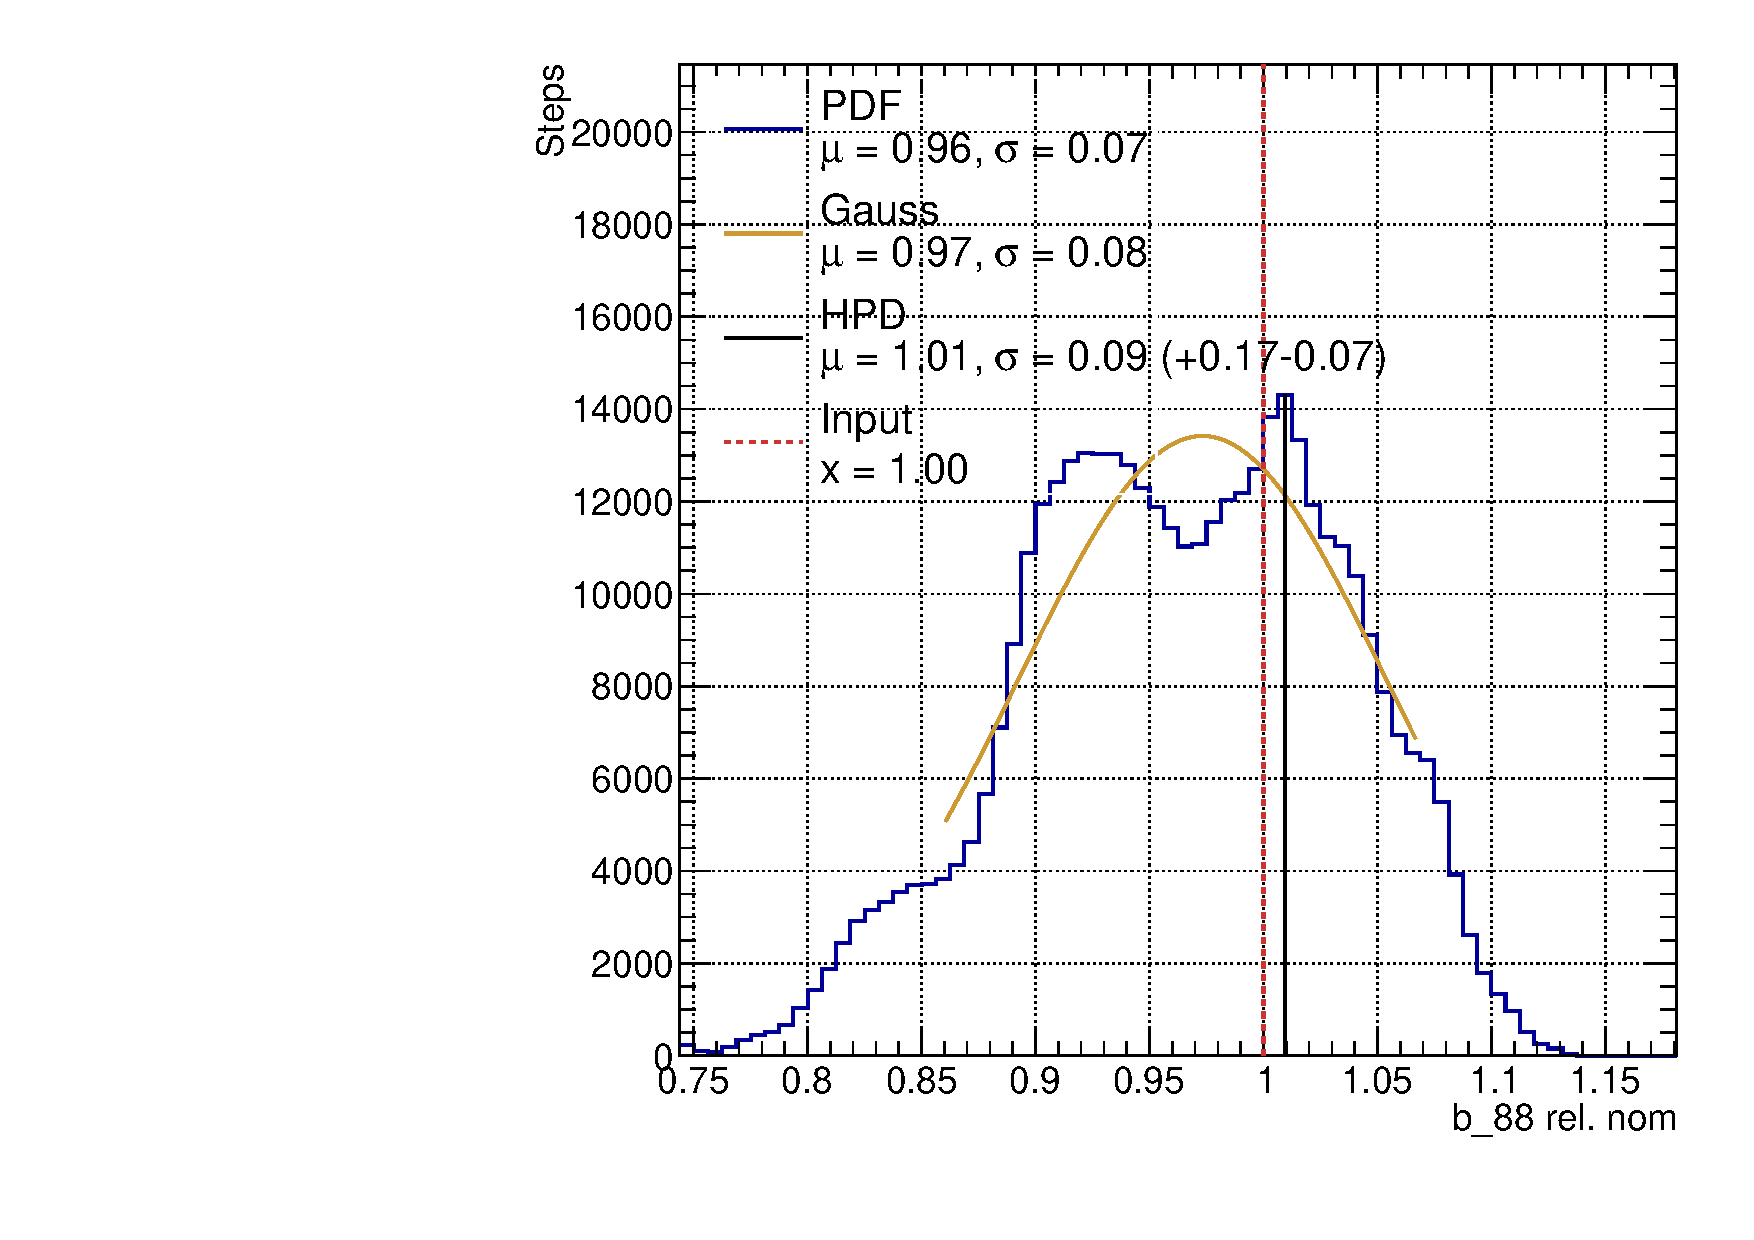
\includegraphics[width=0.6\textwidth, trim={0mm 0mm 0mm 0mm}, clip,page=1]{figures/mcmc/b88_example}
	\caption{One-dimensional marginalised posterior density for a beam parameter, showing three methods of point and error estimation}
	\label{fig:point_estimate}
\end{figure}

In \autoref{fig:point_estimate} we note asymmetric errors in the case of the asymmetric HPD method and different estimates of the central value. Importantly, none of the above methods are de-facto wrong, and in many cases the one dimensional posterior has to be investigated further for e.g. marginalisation effects with other non-Gaussian parameters. Unless otherwise stated, the arithmetic mean and rms are used here due to their simplicity.

\subsection{Covariance Estimates}
In the case of estimating covariances a similar method is used. We marginalise the high-dimensional posterior onto the two parameters whose covariance we wish to calculate. The marginal posterior is binned and the covariance is calculated arithmetically without assuming a shape of the posterior. \autoref{fig:cov_2d_posterior} shows two example two-dimensional marginal posteriors between beam and interaction parameters, one of which results in a strong correlation and the other doesn't.

\begin{figure}[h]
	\begin{subfigure}[t]{0.40\textwidth}
		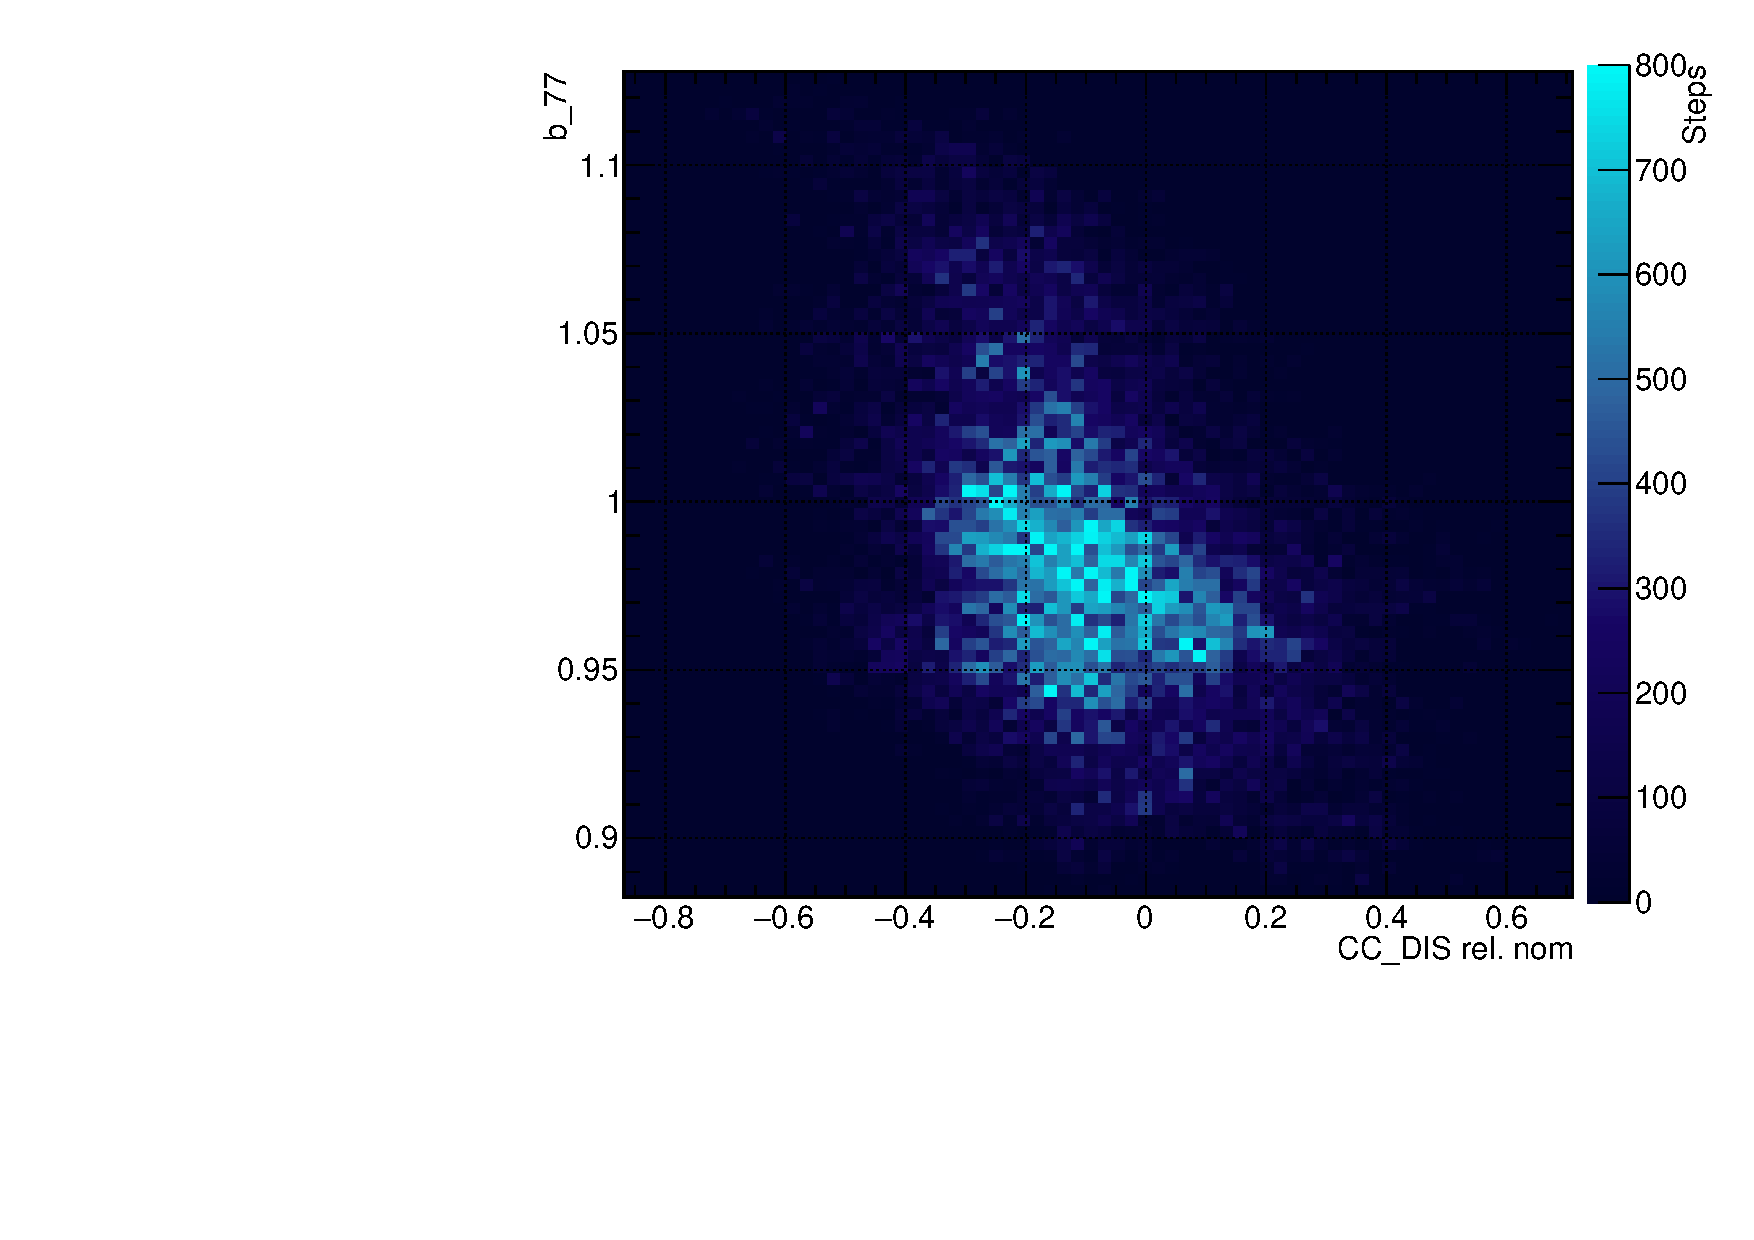
\includegraphics[width=\textwidth, trim={0mm 0mm 0mm 0mm}, clip,page=1]{figures/mcmc/example_corr}
		\caption{Strong correlation}
	\end{subfigure}
	\begin{subfigure}[t]{0.40\textwidth}
		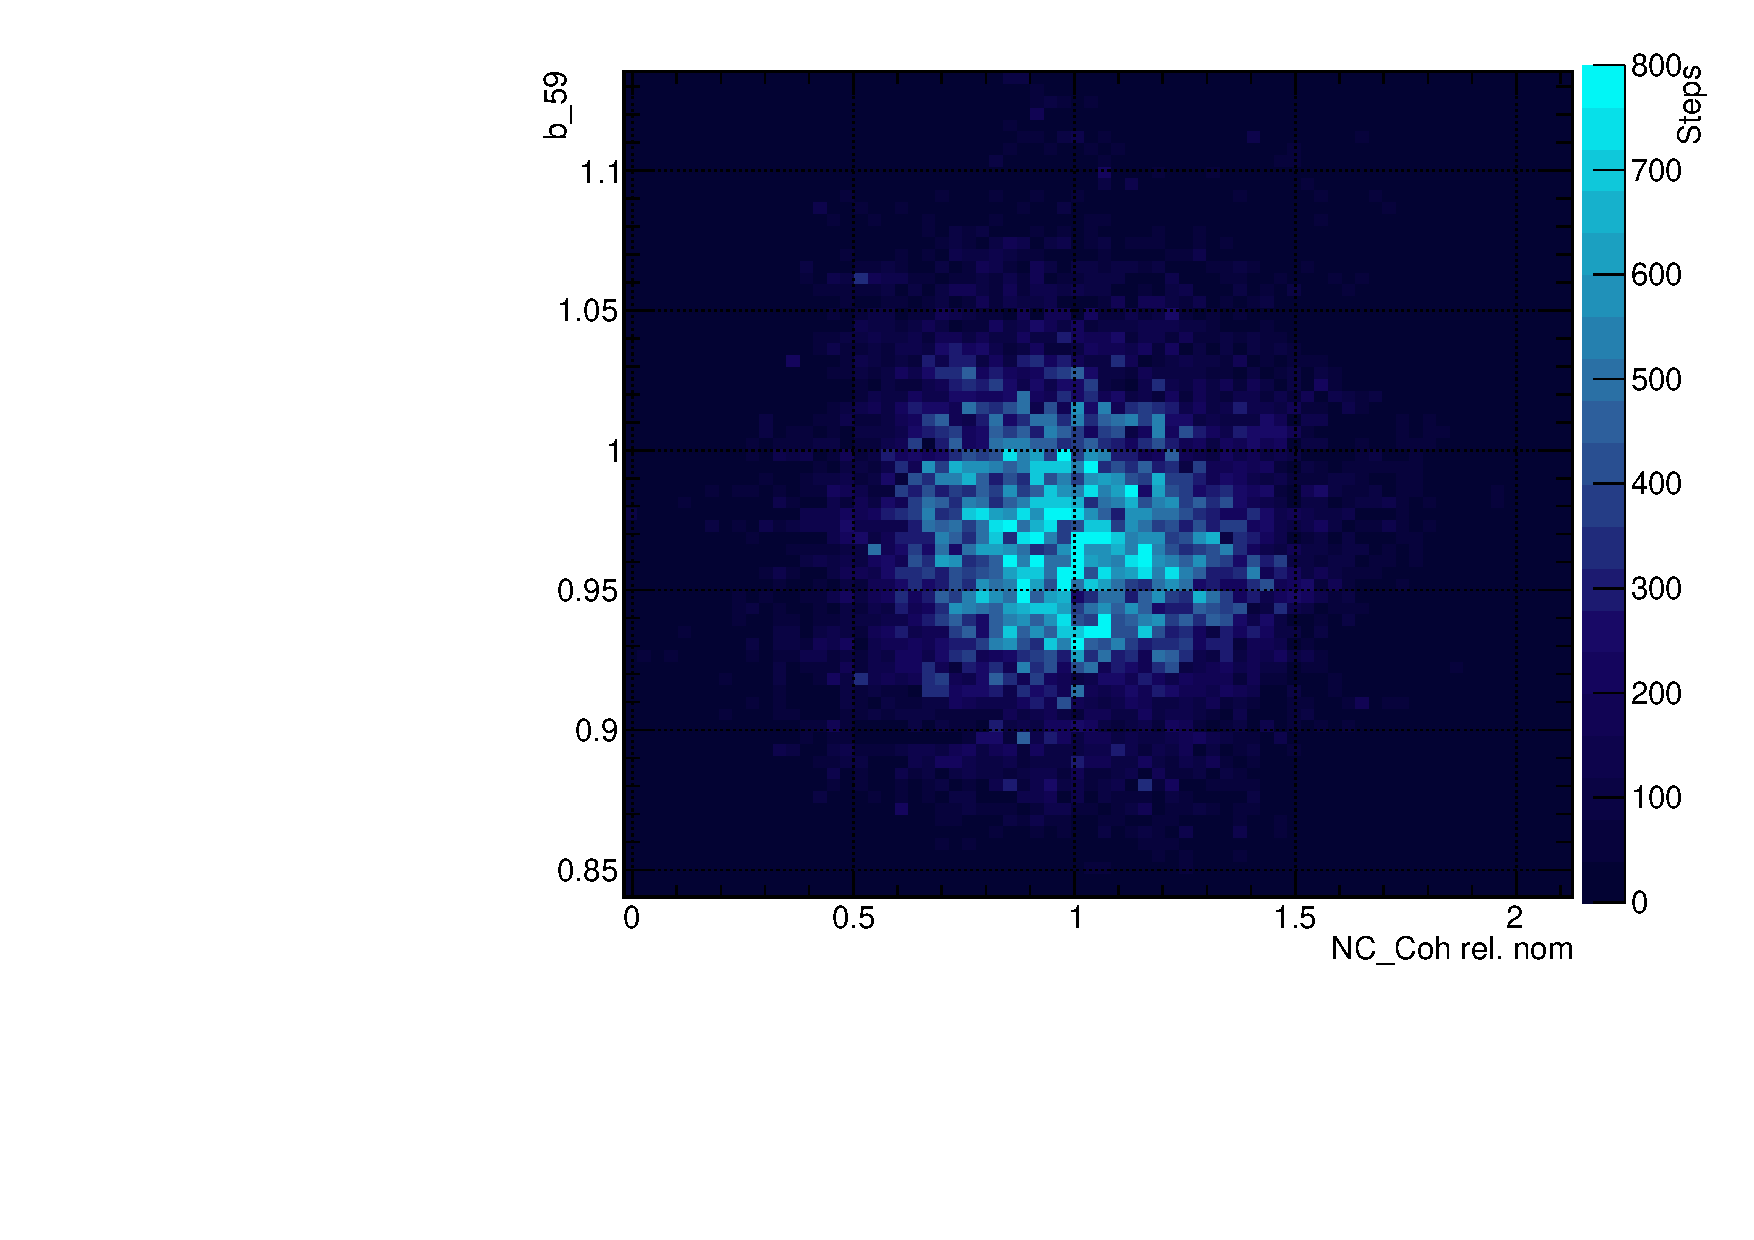
\includegraphics[width=\textwidth, trim={0mm 0mm 0mm 0mm}, clip,page=1]{figures/mcmc/example_corr2}
		\caption{Weak correlation}
	\end{subfigure}
	\caption{Two-dimensional marginal posteriors used to calculate parameter covariance}
	\label{fig:cov_2d_posterior}
\end{figure}

\section{Predictive Checks and p-values}
A Bayesian analysis conditions on the entire model's probability, so can lead to misleading results when the model space strongly disagrees with the data space. Assessing the model goodness against data is therefore critical in any Bayesian analysis, and closely follows what is detailed in \cite{posterior_predictive_checks, posterior_predictive_checks2, posterior_predictive_checks3, prior_predictive_checks}. 

This analysis uses two ``goodness-of-fit'' checks, in which the test-statistic from the statistics of the sample for observed events $n$ with predicted events $\lambda$,

\begin{equation}
	-\log\mathcal{L}_\text{Samples} = \lambda-n+n\log\frac{n}{\lambda}
	\label{eq:sample_stat}
\end{equation}

is of central importance. The ``predictive spectrum'' of a distribution from a model is also crucial, and is defined as having a point estimate $\bar{\lambda}$ equal to the average predicted events over $N$ randomly chosen MCMC steps after burn-in,

\begin{equation}
	\bar{\lambda} = \frac{1}{N} \sum^{N}_i \lambda_i
\end{equation}

with the error $\Delta \bar{\lambda}$ taken as the root mean square,

\begin{equation}
	\Delta \bar{\lambda} = \sqrt{\frac{1}{N} \sum^{N}_i \lambda^2_i}
\end{equation}

For this analysis it was checked that the predictive spectrum using the arithmetic mean and rms were consistent with a Gaussian fit\footnote{Extracting $\bar{\lambda}$ and $\Delta \bar{\lambda}$ from the fitted parameters}, and separately the mode with 68\% central highest posterior density of the bin.

The goodness-of-fit tests involve applying statistical fluctuations to a drawn simulation, calculating the test-statistic in \autoref{eq:sample_stat} of the fluctuation versus some other distribution. Then locating the test-statistic of the posterior predictive spectrum (``best-fit'') given the data gives a $p$ value. The methods are:

\begin{itemize} 
	\item A one-dimensional plot of the test-statistic between the drawn distribution and the statistical fluctuation of that drawn distribution
	\item A two-dimensional plot of the test-statistic between the data and the drawn distribution, versus the test-statistic between a fluctuation of the drawn distribution and the drawn distribution
\end{itemize}
The former case simply locates the realised test-statistic in a distribution, whereas the second informs about the predictive nature of the model after having seen data, were we to observe more data. Formally,

\begin{equation}
P(D'|D_{obs}) = \int P(D'|\vec{\theta}) P(\vec{\theta}|D_{obs}) d\vec{\theta}
\end{equation}

To construct the p-value in the two-dimensional case we need to compare to a reference distribution, which is the statistically fluctuated drawn histogram in this case. In practice, 20,000 random draws of the parameters are performed after burn-in, which samples the posterior. For each draw we
\begin{itemize}
	\item Reweight the Monte-Carlo using the new parameter set
	\item Poisson fluctuate each Monte-Carlo bin according to its bin contents
	\item Calculate the test-statistic between the fluctuated histogram and the drawn histogram, denoted $\chi^2_{\text{Draw, Draw Fluc}}$
	\item Calculate the test-statistic between the observed data and the drawn histogram, denoted $\chi^2_{\text{Data, Draw}}$.
	\item Fill a two dimensional histogram of the two test-statistics
\end{itemize}
The predictive spectrum is formed by taking the mean in each bin as the central number of events, and the error is calculated in the same way. Hence the posterior predictive distribution is not truly observed from one MCMC draw but is rather the distribution representative of the posterior.

The two-dimensional posterior predictive p-value is then finally
\begin{equation}
p = \frac{N\left(\chi^2_{\text{Data, Draw}} < \chi^2_{\text{Draw, Draw Fluc}}\right)}{N\left(\text{Total}\right)}
\end{equation}
where $N\left(\chi^2_{\text{Data, Draw}} < \chi^2_{\text{Draw, Draw Fluc}}\right)$ is the number of times a drawn distribution had a smaller test-statistic against data than it did against a fluctuation of itself, and $N(\text{Total})$ is the total number of draws.

The p-values are also used for statistical closure tests, where the drawn distribution is instead the predictive distribution. Furthermore, the drawn distribution can be from both the prior and posterior densities.